% Homework Template
\documentclass[a4paper]{article}
\usepackage{ctex}
\usepackage{amsmath, amssymb, amsthm}
\usepackage{moreenum}
\usepackage{mathtools}
\usepackage{url}
\usepackage{bm}
\usepackage{enumitem}
\usepackage{graphicx}
\usepackage{subcaption}
\usepackage{booktabs} % toprule
\usepackage[mathcal]{eucal}
\usepackage[thehwcnt = 6]{iidef}
\usepackage{float}
\usepackage[sort]{natbib}

\thecourseinstitute{清华大学电子工程系}
\thecoursename{\textbf{媒体与认知} \space 课堂2}
\theterm{2021-2022学年春季学期}
\hwname{作业}

\begin{document}
\courseheader
\name{郭中贺}
\vspace{3mm}
\centerline{\textbf{\Large{调研报告部分}}}
\vspace{3mm}

\section{关于媒体与认知技术在新冠肺炎诊断方面应用的调研报告}
\subsection{问题背景}
\hspace{2em}自新冠疫情爆发以来,人们的生活与工作受到了很大影响,在医疗科学领域,如何精确而正确地诊断新冠肺炎是一个重要问题。\cite{111}指出,到目前为止,X射线扫描和CT为诊断肺部疾病的首要检查方法,然而肺部影像不仅有着复杂的表现,而且目前我国肺部影像的数据量逐年增长,多种因素导致影像科医生任务繁重。因此,为了解决这种医疗问题,基于人工智能的疾病诊断技术应运而生,为医学影像检查提供了广阔应用前景。
\subsection{已有措施与技术}
\hspace{2em} \cite{222}研究人员,一方面通过肺叶分割和联合执行严重度评估,进而对原始三维 CT 图 像中的新冠肺炎严重度进行自动评估。另一方面,他们开发了一个多任务、多实例 M2UNET 网络评估新冠肺炎患者的严重程度。\\
\hspace{2em}\cite{333}研究人员利用基于深度学习的AI模型实现肺炎病灶的自动分割,从每一帧图像的病灶区域中提取影像组学特征,经过LASSO回归降维后分别采用高斯朴素贝叶斯、随机森林和极端梯度提升的方法在训练集中建立影像组学模型,并在验证集中测试模型性能。采用Dice系数评估肺炎病灶分割的准确性,采用ROC评估新冠肺炎诊断效能。
\subsection{技术效果分析}
\hspace{2em}在肺炎病灶分割方面,需要以人工标记结果为标签,利用图像处理方法以及深度学习来实现对CT影像中验证病灶的自动分割,研究人员的结果也表明,AI分割的病灶与人工标记结果有着非常好的一致性。\\
\hspace{2em}对于提取的影像组学特征,我们可以使用一些方法对特征进行降维,保留关键信息,去除冗余信息。\\
\hspace{2em}之后,我们可以基于提取的特征,来对CT图像进行新冠肺炎的结果诊断学习,徐翠莲等研究人员的实验也证明,基于高斯朴素贝叶斯的模型获得了相对较好的效能,其模型在薄层CT影像验证集上的AUC分别为0.919、0.838和0.829,在厚层CT影像验证集上的AUC分别为0.802、0.730和0.715。
\subsection{未来优化思路}
\hspace{2em}虽然目前人工智能在上述医疗方面发挥了重要的作用,但是由于技术原因和其他因素的制约,还存在一定的问题。例如,基于机器学习的方法对医学影像进行诊断必定要基于大量的数据,否则学习效果不能使人满意。而这些医学影像作为数据输入时,通常需要提前进行人工标注。因此,在未来的工作中,我们需要建立更加完善的医学影像数据库,从而有效提升图像的临床代表性、标注规范性与图像多样性。另一方面,我们还可以进一步开发半监督甚至无监督的学习模型来对医学影像进行诊断,提高算法的泛用性。
\vspace{3mm}
\centerline{\textbf{\Large{编程部分}}}
\vspace{3mm}
% 请根据是否选择自选课题的情况选择“编程作业报告”或“自选课题开题报告”中的一项完成
\section{编程作业报告}
\subsection{代码补全}
\hspace{2em}补全代码后,运行命令python network.py,以验证代码的正确性。结果如下:\\
\begin{figure}[H]
    \centering
    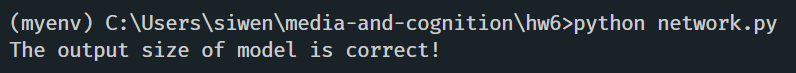
\includegraphics[width=8cm]{1.png}
\end{figure}
\hspace{2em}如图,可以看出网络输出变量的尺寸是正确的,可以看出 Transformer 层
实现完成。
\subsection{模型训练}
\hspace{2em}输入如下命令:python main.py –mode train 进行训练100轮,得到
训练结果如下:\\
\begin{figure}[H]
    \centering
    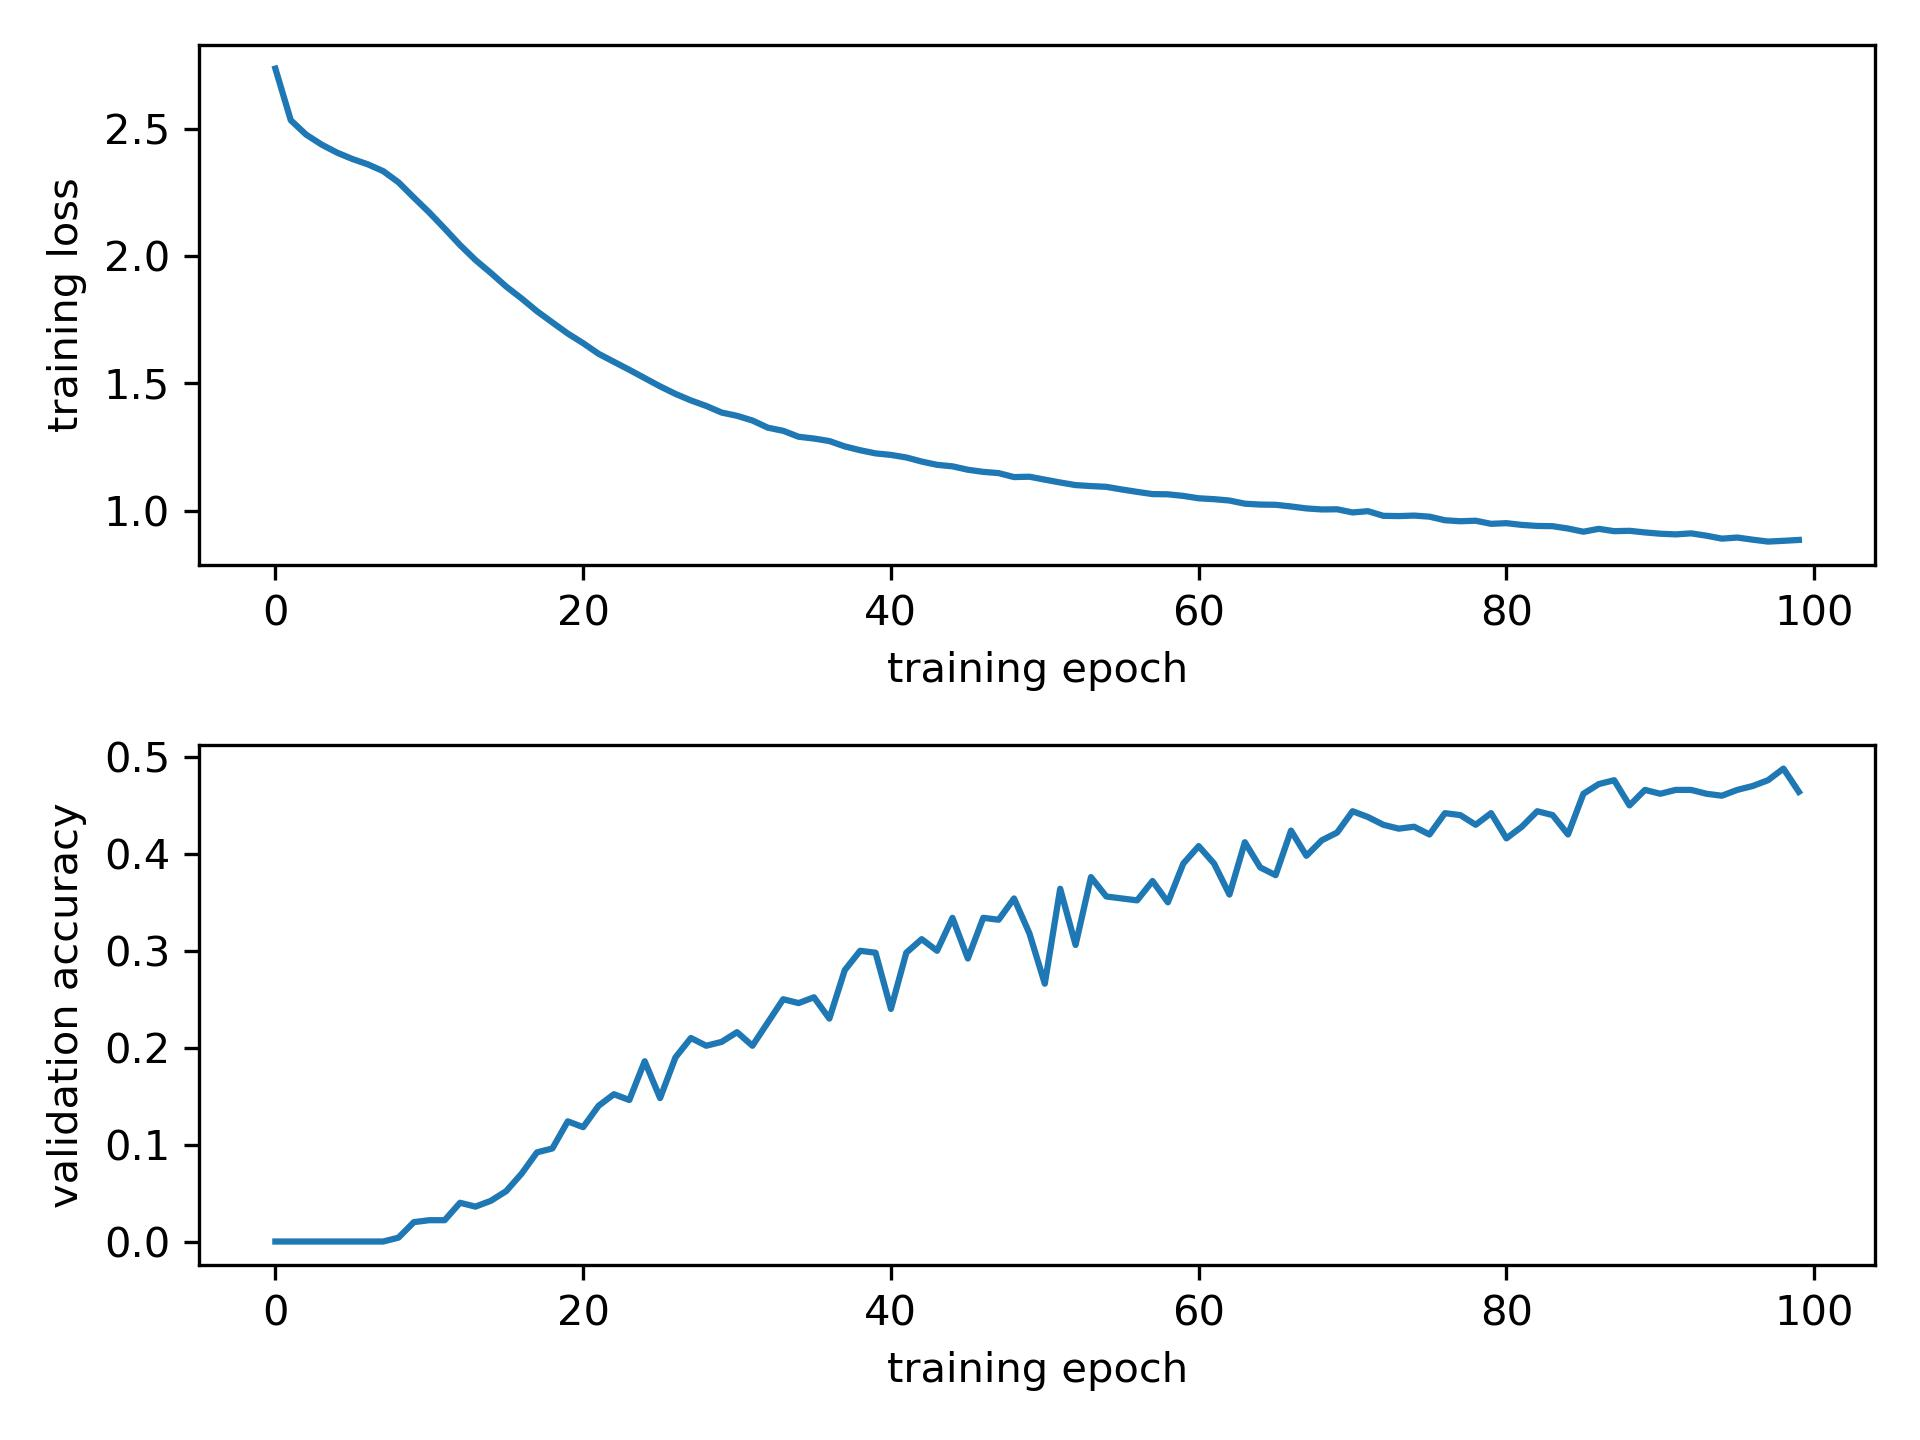
\includegraphics[width=8cm]{loss_and_accuracy_100.jpg}
\end{figure}
\hspace{2em}可以看到,训练完成100轮后,模型在验证集上的loss降低到0.8左右,准确率较低,但也达到了50\%左右。\\
\hspace{2em}使用命令 python main.py --mode train --load\_pretrain --pretrain\_path models/model\_epoch100.pth --epoch 10 将模型继续训练10轮之后,得到结果如下:\\
\begin{figure}[H]
    \centering
    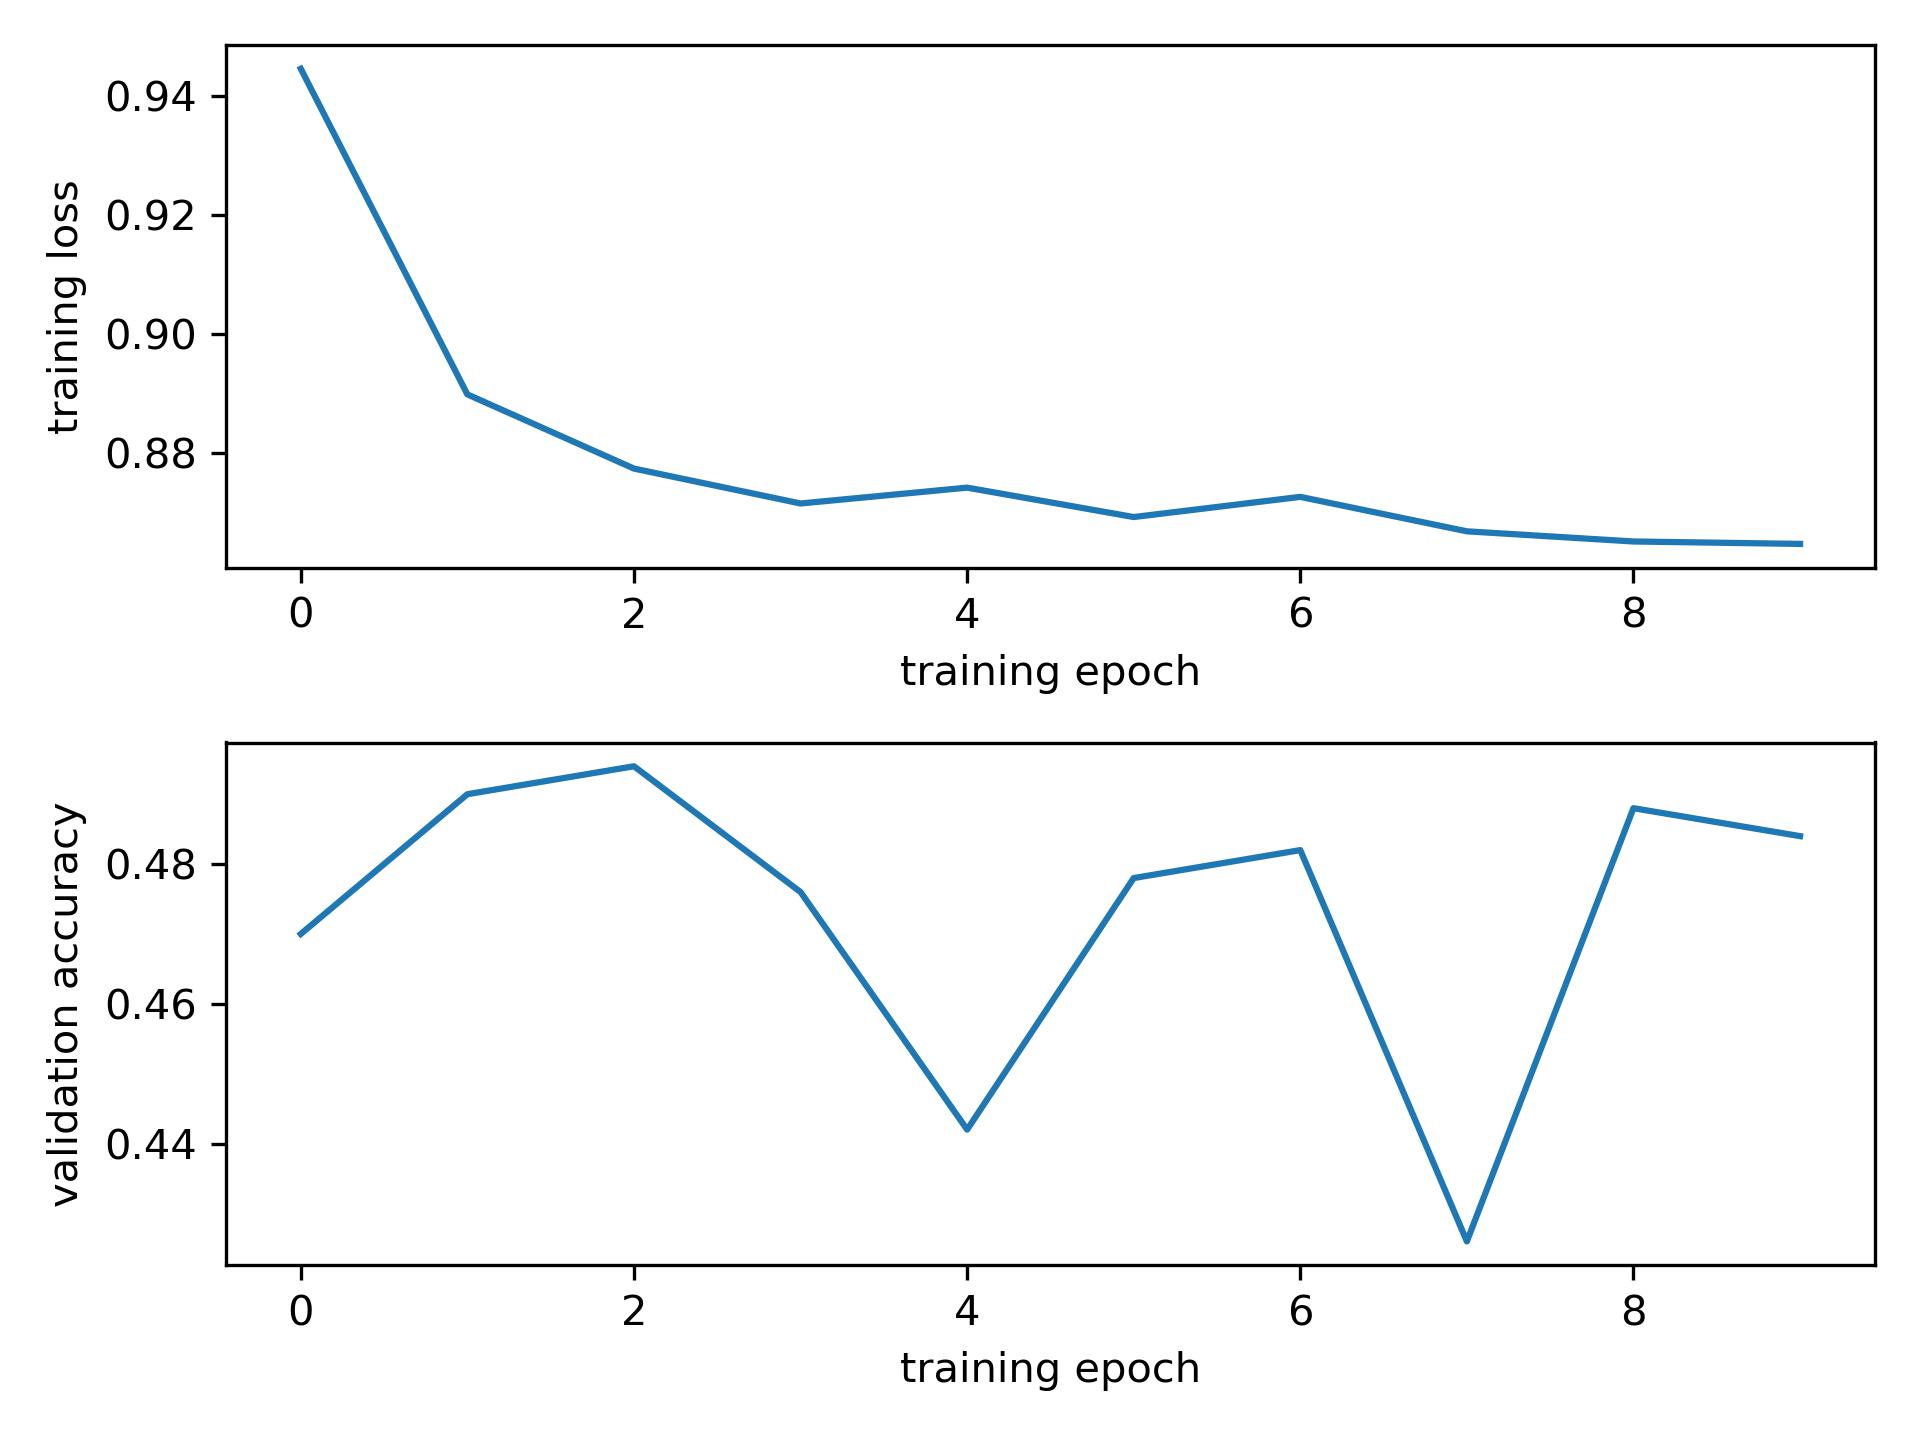
\includegraphics[width=8cm]{loss_and_accuracy.jpg}
\end{figure}
\hspace{2em}其中最后一轮的loss和accuracy分别为0.865和48.4\%:
\begin{figure}[H]
    \centering
    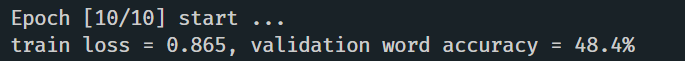
\includegraphics[width=8cm]{2.png}
\end{figure}
\hspace{2em}由于我们使用的
数据量较小所导致的最终在验证集上的正确率大概只有 50\% 左右,从 loss
和 accuracy 变化曲线中我们可以发现,训练初期由于模型在学习过程中,
初期的 loss 下降较慢,准确率也一直为 0,而随着训练的逐渐进行,大概从
第 10 轮开始,准确率开始逐渐上升,到 80 轮之后,
loss 下降速度减缓,准确率上下波动开始较为明显。
总的来说,训练的结果还是较为理想的。可以看出,与上次作业中采用 RNN 网络模型相比,该次训练过程要更加困难,这与 transformer 本身特性有关。\\
\hspace{2em}
\textbf{transformer 在训练时具有并行训练的特性,原因在于}
其自注意的机制,在解码时每个时刻的输入
依赖的是正确的样本,而非上一时刻的输出。
transformer 实现 Decoder 部分训练并行化,就是一次性将整个目标句子输
入给 decoder,然后利用自注意力算法计算出结果,往后面网络继续传递,
最后计算出预测值,分别对应每个时刻的输出,从而实现并行训练。
\subsection{使用训练好的模型预测新的文本图像}
\hspace{2em}使用命令 python main.py --mode predict --im\_path data/my\_own/recommend.png,
预测新的文本图像。输入图像为:\\
\begin{figure}[h]
    \centering
    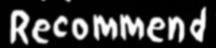
\includegraphics[width=8cm]{recommend.png}
\end{figure}
\hspace{2em}使用上面一共训练110轮的模型进行预测。
输出结果如下:\\
\begin{figure}[h]
    \centering
    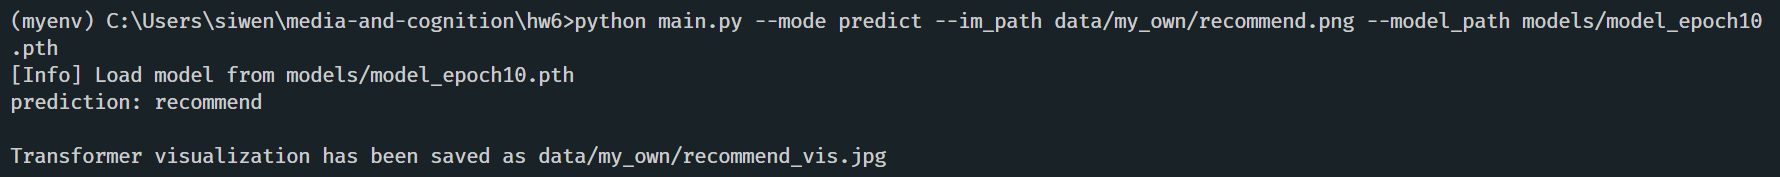
\includegraphics[width=10cm]{3.png}
\end{figure}
可视化结果如下:\par
\begin{figure}[H]
    \centering
    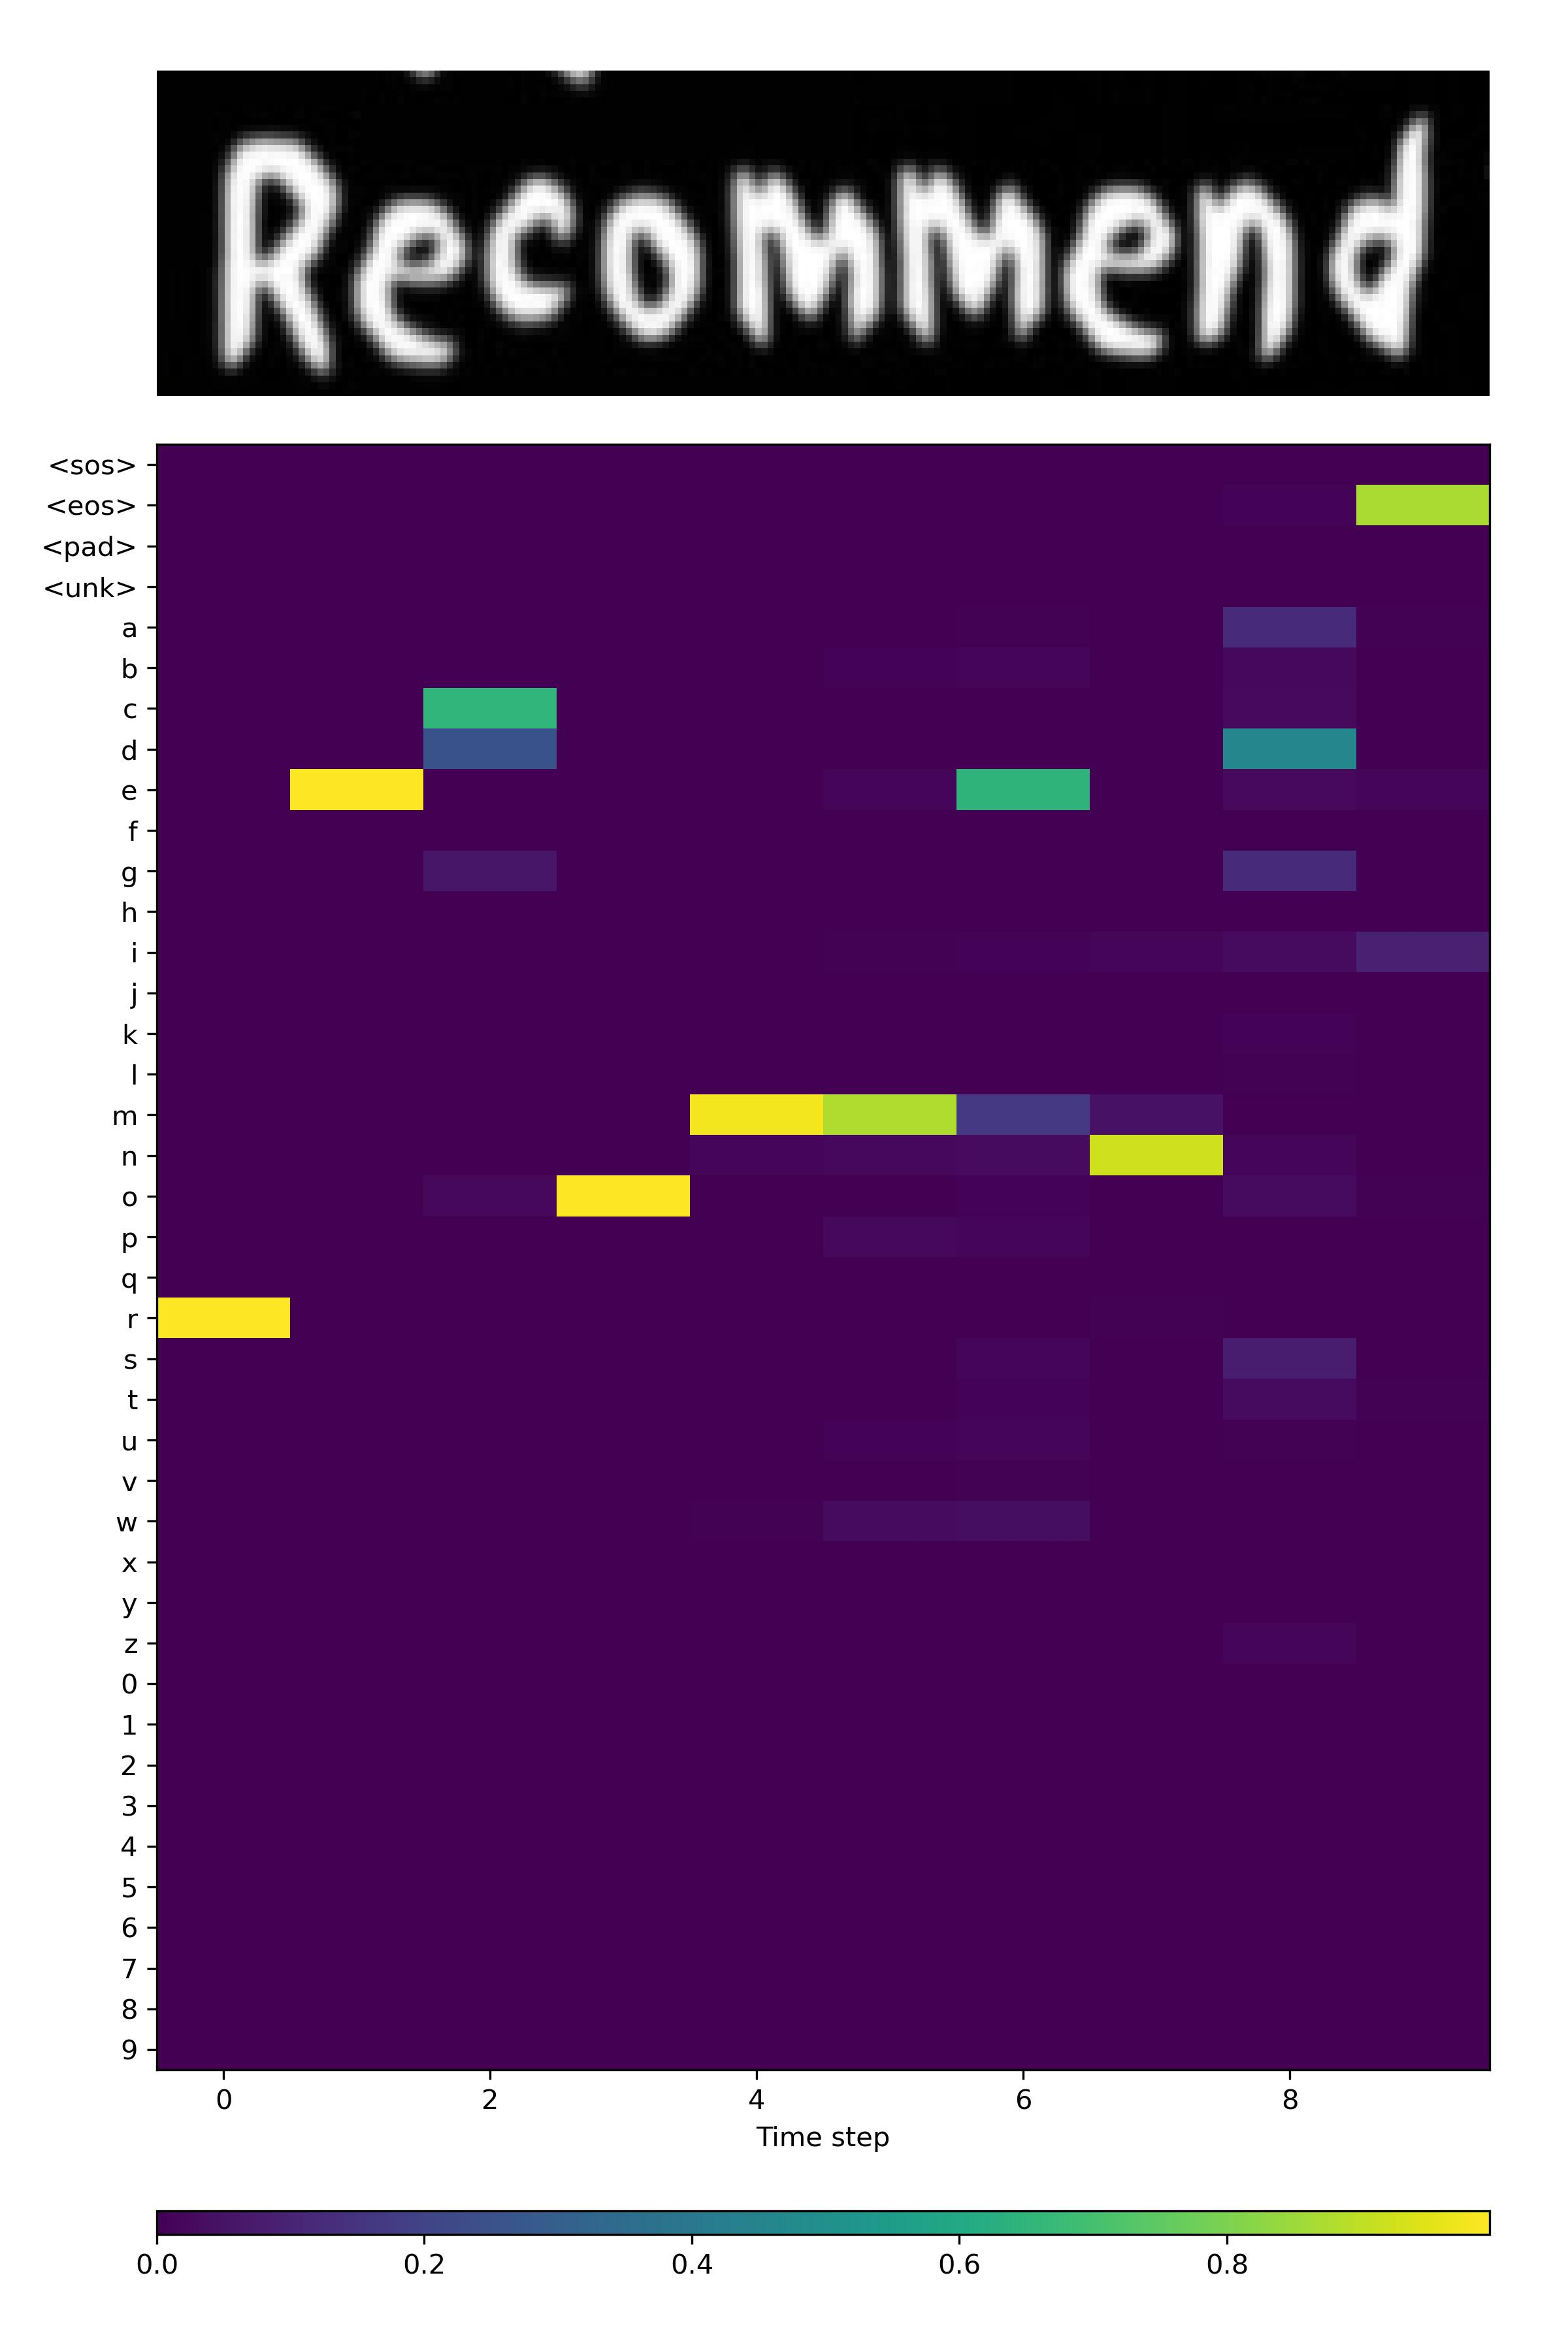
\includegraphics[width=10cm]{recommend_vis.jpg}
\end{figure}

\hspace{2em}可以看到得到了正确的预测结果 recommend,结合可视化结果我们可以看
到这里预测的结果为recommend-,.能够正确识别,一方面是由于输入图像较为理想,
字符清晰易分辨,另一方面也可以看出模型有一定的泛用性。
上一次的作业的可视化结果中,我们发现不同字母之间通常会间隔一个或多个空白符,
通过CTC解码可以得到正确的结果。而本次作业使用的transformer解码,能够直接输出正确字符序列。\\

\hspace{2em}\textbf{更进一步地说,transformer 解码和 CTC 解码的区别在于:}
Transformer 是属于 Attention-based 的模型,通过注意力机制对各个输入进行联合建模
需要一次获取整个输入语音编码序列。在 Decoder 的时候,是需要根据之前的翻译,求解当前最有可能的翻译,
CTC 则是基于条件独立性假设,每个时刻的输出仅依赖于当前时刻的输入,不需要等待完整的上文输入,通过引入空白符的方式,保持输入与输出的单调对齐,使用动态规划的算法实现快速的解码。

\subsection{本次作业遇到的问题及解决方法}
无。
\subsection{对本次作业的意见及建议}
本次作业也较为简单,通过代码注释中的一步一步教程,
我们能很快了解下一步该做什么,该如何实现,感谢老师和助教的悉心指导
\bibliographystyle{thuthesis-numeric}
\bibliography{refs}  % 参考文献使用 BibTeX 编译

\end{document}



%%% Local Variables:
%%% mode: late\rvx
%%% TeX-master: t
%%% End:
